\documentclass[12pt]{article}


\newcommand{\ttt}{\texttt}

\usepackage[english]{babel}
\usepackage[utf8]{inputenc}
\usepackage{amsmath}
\usepackage{amssymb}
\usepackage{gensymb}
\usepackage{graphicx}
\usepackage[colorinlistoftodos]{todonotes}
\usepackage{color}
\usepackage{minted}
\usepackage{fullpage}
%\usepackage{undertilde}
\usepackage{accents}
\usepackage{bigints}
\usepackage{verbatim}
\usepackage[super]{nth}
\usepackage{listings}
\usepackage[margin=0.7in]{geometry}
\usepackage{courier}
\usepackage{epstopdf}
\usepackage{placeins}
\usepackage{lipsum}
\usepackage{subfig}
\usepackage{booktabs}
\usepackage{hyperref}
\usepackage{textcomp}

\title{Paralle Unstructured Mesh Interface: Terminology and Structure}
\author{Jared Crean}
\date{June 21, 2015}
\begin{document}
\maketitle

\tableofcontents

\section{What is PUMI}
PUMI stands for Parallel Unstructures Mesh Interface.  It is useful for interacting with the mesh for performing Finite Element analysis.  PUMI stores more information than classic mesh software, which allows some operations to be performed much faster than is possible using only the information stored by classic mesh software.

The organizing principle of PUMI is that mesh information is stored as a graph.  A graph is a description of how objects are related to each other.  PUMI stores a mesh as a 4 dimensional graph, which is to say it stores the relationships between vertices, edges, faces, and regions (3d figures).  PUMI allows the user to access this information, which in turn allows the user carry out a Finite Element analysis.  

The paragraph above describes the core functionality of PUMI.  PUMI also has some additional functionality which is useful.  PUMI organizes data in a 3 level hierarchy. Meshes are often created from CAD models, so PUMI has added the capability to access geometry information on how the mesh relates to the geometry.  Further, PUMI has added the ability to create fields on top of the mesh.  To understand the distinction between the mesh and a field, let's be specific about what the mesh is.  The mesh describes the size and shape of the elements.  It says nothing about nodes.  The nodes are an example of a field.  In general, a field is data that is stores in a way that references the mesh.  The nodes are a field because the locations of nodes are defined relative to the vertices, edge, faces, and regions of the mesh.

To summarize, PUMI has a 3 level scheme:

Geometry - Mesh - Field

We will be more specific about the relationships between these levels later.


\section{Terminology}
To begin, let's define the terminology PUMI uses to describe the mesh and the objects it is composed of.  A term will be \textbf{bolded} when it is defined.  Thereafter, all uses of the word refer to the definition introduced here.

A \textbf{mesh} is composed of \textbf{mesh entities}.  The dimensions of mesh entities are \textbf{vertex}, \textbf{edge}, \textbf{face}, \textbf{region}.  The \textbf{dimension} of a mesh entity describes the mathematic dimensionality of the object.  Vertices have dimension zero, edges have dimension one, faces have dimension two, and regions have dimension three. Each mesh entity also has a \textbf{type}, which describes the geometric shape of the mesh entity.   The type of mesh entity is more specific than the dimension, in that there can be multiple types for an entity with a given dimension.  The possible types are vertex, edge, triangle, quad, tet, hex, prism, and pyramid.  Note that a 2d entity could either be a triangle or a quad (quadralateral), and a 3d entity could be any of tet (tetrahedron), hex (hexahedron), prism (wedge shape), or pyramid.  The regions supported by Pumi are shown in figures \ref{fig:vert_ordering} and \ref{fig:edge_ordering}.


\begin{figure}
\centering
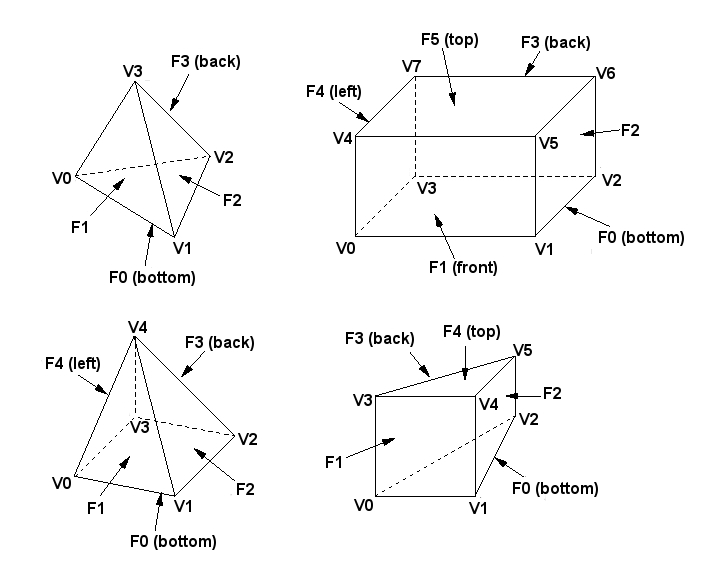
\includegraphics[width=0.75\textwidth]{region_faces.jpg}
\caption{\label{fig:vert_ordering} Vertex and Face Ordering  }
\end{figure}

\begin{figure}
\centering
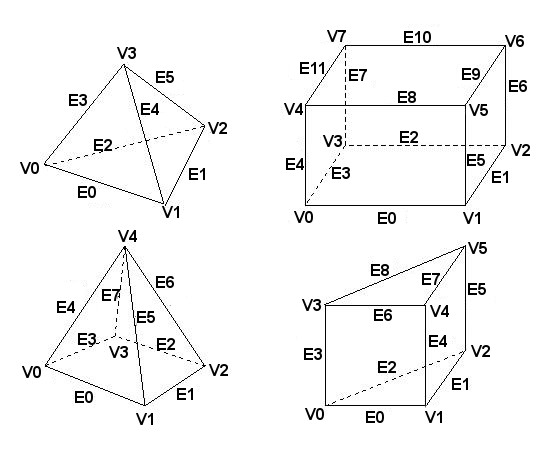
\includegraphics[width=0.75\textwidth]{region_edges.jpg}
\caption{\label{fig:edge_ordering} Vertex and Face Ordering  }
\end{figure}

\FloatBarrier

% INCLUDE PICTURES FROM DOCUMENTATION HERE

Two mesh entities are said to be \textbf{adjacent} if directly connected in the 4d graph of the mesh.  More simply, if one entity is part of the other, then they are adjacent.  For example, a vertex and an edge are adjacent if the vertex is part of the edge.  Similarly, a vertex and a face are adjacent if the vertex is part of the face.  Note that adjacency is bi-directional.  If a vertex is adjacent to an edge, then the edge is adjacent to the vertex.  Mesh entity x is said to be \textbf{upward} adjacent to mesh entity y is the dimension of x is greater than the dimension of y.  Similarly, x is \textbf{downward} adjacent to y if the dimension of x is less than the dimension of y. A mesh entity is not adjacent to itself.

The PUMI documentation uses these terms for variable names, and often times that will be the only clue as to what value to use.

When talking about fields , it is convenient to describe a field entity being \textbf{classified} on a mesh entity.  This means that the field entity is described relative to the mesh entity.  This is important to know when trying to access field data because it reflects the data structure used to store it.

\section{Organization of APF}
This section descrbes the Attached Parallel Fields (APF) interface that we use to interact with PUMI.  Useful functions from each class or header file will be discussed below.

The class \ttt{apf::Mesh} contains functions used to access the mesh and mesh entities.  
Its primary purpose is to allow querying of adjacency information.  The class \ttt{apf::Mesh2} contains all the functionality of \ttt{apf::Mesh} plus the ability to create meshes.  
The header \ttt{apfShape.h} defines classes and functions to describe nodes and shape functions.  
The classes it defines are called \ttt{apf::FieldShape} and \ttt{apf::EntityShape}.
The file \ttt{apfNumbering.h} contains functions for assigning numbers to mesh entities and degrees of freedom (dof).

\section{apf::Mesh}
The purpose of the mesh class is to enable querying of adjacency information.  
Before describing how it does that, first we need to understand how PUMI allows the user to access the mesh.
PUMI defines a datatype called an \ttt{apf::MeshEntity*}, which is a pointer to a mesh entity of some kind.  It can point to any kind of mesh entity, which is to say any vertex, edge, face, or region.
This is helpful because statically typed languages like C++ would normally require a variable of a different type to access the different types of mesh entities, but using \ttt{apf::MeshEntity*} we can write code that works for any kind of mesh entity.
There is a function which is in the apf namespace but is not a member function of \ttt{apf::Mesh} with signature  
\newline
\newline
\noindent\texttt{int getDimension(apf::Mesh *m, apf::MeshEntity* e)} 
\newline
\newline
\noindent that returns the dimension of the mesh entity.  
There is also a member of the \ttt{apf::Mesh} with signature 
\newline
\newline
\noindent\ttt{int getType(MeshEntity* e)} 
\newline
\newline
\noindent that returns an integer describing the type of the mesh entity.  
The integer is actually an enum, so it should not be necessary to know the meaning of the integer (the values can be accessed using \ttt{apf::TYPE\_NAME}, but it is helpful some times, so it is defined in table \ref{tab:type_enum}).


\begin{table}[h]
\centering
\begin{tabular}{@{}|l|l|@{}}
\toprule
Value & Meaning       \\ \midrule
0     & Vertex        \\ \midrule
1     & Edge          \\ \midrule
2     & Triangle      \\ \midrule
3     & Quadralateral \\ \midrule
4     & Tetrahedron   \\ \midrule
5     & Hex           \\ \midrule
6     & Prism         \\ \midrule
7     & Pyramid       \\ \bottomrule
\end{tabular}
\caption{Mesh Entity Type Enumeration}
\label{tab:type_enum}
\end{table}

So, how do we get a pointer to a mesh entity if we don't already have one?  
The answer is iterators.  
PUMI has iterators over the mesh entities that allow you to access individual mesh entities, and work just like C++ Standard Template Library iterators (if you are unfamiliar with the concept of iterators, consult a book on C++, Lippman's C++ Primer is a good choice). 
You create an \ttt{apf::MeshIterator*} over mesh entities of a particular dimension using
\newline
\newline
\noindent\ttt{apf::MeshIterator* begin(int dimension)} 
\newline
\newline
\noindent The function 
\newline
\newline
\noindent\ttt{MeshEntity* iterate(MeshIterator* it)}
\newline
\newline
\noindent returns a pointer to the current mesh entity and advances the iterator to the next one.  
It is your responsibility to not call \ttt{iterate} on the pointer when it is pointing to the last mesh entity, and you will get an error if you do so by mistake.  
When the result of this funciton is cast into a bool, it returns true if it is safe to call the function again, and false if the iterator is pointing to the last mesh entity.
This makes in convienient iterate over all mesh entities of a certain type using a \ttt{while} loop.
When the iterator reaches the end, you have to destroy the old iterator with the function \ttt{end} get a new one using \ttt{begin}.

Now that you can get mesh entity pointers, how do we get adjacency information?  
We use the function \ttt{getDownward} and \ttt{getAdjacent}. 
These functions have signatures:
\newline
\newline
\noindent\ttt{int getDownward(MeshEntity* e, int dimension, MeshEntity** adjacent)}

\noindent\ttt{void getAdjacent(MeshEntity* e, int dimension, Adjacent\& adjacent)}
\newline
\newline
Lets talk about downward adjacencies first.  The \ttt{getDownward} function takes in the mesh entity you want to get the adjacent entities of, the dimension of the entities you want to retrieve, and an array to store their pointers in.
The array can be a standard C array, or it can be an array of type apf::Downward.  The array should be of size 12, because that is the maximum number of downward adjacencies any mesh entity can have. Only the first $n$ entries of the array are used.  The integer returned by \ttt{getDownward} is $n$.
The entries in the array are guaranteed to be ordered according to the canonical ordering in figures \ref{fig:vert_ordering} and \ref{fig:edge_ordering}.  One way to conceptualize the ordering is that the entire figure is defined by the vertices.  The first edge is always between the first and second vertices, the first face is always defined by the first 3 or 4 vertices, depending on whether the face is a triangle or quadralateral.
The definition of the vertices (ie. which vertex is vertex 0, which one is vertex 1 etc.) is determined at mesh creation time.  This is important to know if you are interested in determining the relative alignment of the elements.
That's all there is to downward adjacencies.  They are relatively simple because the number of downward adjacencies is known ahead of time.

Upward adjacencies are a bit more complicated because, for an unstructured mesh, the number of upward adjacencies is not known a priori.  The first two arguments to \ttt{getAdjacent} are the same as \ttt{getDownward}.  
The final argument is different, an array of type \ttt{apf::Adjacent}, which is an alias for a \ttt{DynamicArray<MeshEntity*>}.  It is a dynamically resizeable array, which is exactly what is needed because PUMI doesn't know how many mesh entities it needs to return until it goes and fetches them.
\ttt{DynamicArray} has a member function \ttt{getSize}, which returns the size of the array.   You can use this to find out how many adjacencies are returned because \ttt{getAdjacent} makes the array the exact size it needs.
Unlike downward adjacencies, the mesh entities returned here are in no particular order, which makes using them in algorithms more difficult.

Another useful feature of \ttt{apf::Mesh} is tags.
Tags are a field that allow you to attach arbitrary data to mesh entities. The function
\newline
\newline
\noindent\ttt{MeshTag* createDoubleTag(const char* name, int size)}
\newline
\newline
creates a new tag field, which means it attaches an array of the specified size, of type double, to every mesh entity. 
To put data in the tag of a particular mesh entity, use the function
\newline
\newline
\noindent\ttt{void setDoubleTag(MeshEntity* e, MeshTag* tag, double const* data)}.
\newline
\newline
This function copies \ttt{data} into the array created by the tag field \ttt{tag} of the mesh entity \ttt{e}.  Data is retrieved using the function
\newline
\newline
\noindent\ttt{void getDoubleTag(MeshEntity* e, MeshTag* tag, double* data)},
\newline
\newline
which copies the data from the tag into the array \ttt{data}.
These functions illustrate one of the key features of fields.
The information in the field is only accessible with reference to the mesh.
A particular mesh entity must be passed in to set or retrieve information, and there is no other way to access the data.  
This is a driving principle in how programs that use PUMI are structured.

There are similar functions to create fields with data of type Int and Long.
For storing degree of freedom numbers (performing the function of an IEN array), the \ttt{apf::Numbering} interface is also available and is more convienient for that particular purpose.

The final mesh topic mentioned here is geometric classification.  In addition to the relationship between mesh entities, PUMI also knows the relationship between mesh entities and the geometric entities on the original CAD model.  The function
\newline
\newline
\noindent \ttt{ModelEntity* toModel(MeshEntity* e)}
\newline
\newline
\noindent takes a mesh entity and returns the geometric \ttt{ModelEntity*} that the mesh entity is classified on.  The functions
\newline
\newline
\noindent\ttt{int getModelType(ModelEntity* e)}
\newline
\noindent\ttt{int getModelTag(ModelEntity* e)}
\newline
\newline
tell the dimension of the model entity and the number of the model entity, respectively.
The combination of these two facts uniquely identity a model entity, which is to say that the model number is unique among all model entities of the same dimension, but there might be a model entity of a different dimension with the same number.  
These functions allow querying of the relationship between the mesh and the geometry, which can be useful for operations such as applying different boundary conditions to different parts of the mesh.

\section{apfShape.h}
This header file defines all the functions and classes you need to describe the nodes of the mesh and access shape function values and derivatives.
The class \ttt{apf::FieldShape} describes the locations of the nodes on an element.
The first function that describes node locations is 
\newline
\newline
\noindent\ttt{int countNodesOn(int type)}.
\newline
\newline
The value returned by the function tells the number of nodes classified on mesh entities of the specified type.  Nodes are always classified on the lowest dimension entity possible.  
For example, linear meshes have one node on each vertex, but none on edges, faces, or regions.  
Quadratic (serendipity) mesh have nodes on both one node on each vertex and and one on each edges, but none on faces and regions.  
The argument to this function is the integer type, so if you ask how many nodes are on a quadratic triangle, the answer will be zero, because there are no nodes classified on the faces in a quadratic mesh.  
If you ask for the number of nodes on a vertex, it will tell you 1 for a standard linear mesh.
A complementary function,
\newline
\newline
\noindent\ttt{bool hasNodesIn(int dimension)},
\newline
\newline
determines if there are nodes on entities of a specified dimension.
The function 
\newline
\newline
\noindent\ttt{void getNodeXi(int type, int node, Vector3\& xi)}
\newline
\newline
returns the paramentric coordinates of the specified node on an entity of the specified type in the vector \ttt{xi}.  
There are a couple of important notes about this function.  The first is that is uses parametric coordinates.  For triangular types, it uses barycentric coordinates and for quadralaterals it uses cartesian.  
The second is that it supplies the coordinates in the coordinate system of the specified type, using the minimum number of linearly independent coordinates.
For a node at the centroid of a triangle, for example, the xi vector will read (1/3, 1/3, 0), because the first two coordinates are 1/3 and the final one is not used because it is linearly dependent on the first two.
For the node on the middle of an edge, the xi vector will read (0, 0, 0) because an edge is a one dimensional entity, so it only uses the first coordinate, and the standard parametric coordinate system is the domain [-1, 1], so a mid edge node has coordinate zero.
As you might expect, a node on a vertex is always at (0, 0, 0) because it has no coordinate system being a zero dimensional entity.  
Alternatively, you can think of it as being at the origin of whatever coordinate system it uses.

The last function in \ttt{apf::FieldShape} is 
\newline
\newline
\noindent\ttt{EntityShape* getEntityShape(int type)},
\newline
\newline
which returns a pointer to the \ttt{apf::EntityShape} for the specified type, which gives access to the shape functions.  Each type of entity has its own \ttt{apf::EntityShape} class, because each type of mesh entity has different shape functions.  \ttt{apf::EntityShape} has three functions worth mentioning here.  They are:
\newline
\newline
\noindent\ttt{void getValues(Mesh* m, MeshEntity* e, Vector3 const \&xi, NewArray<double>\& values)}

\noindent\ttt{void getLocalGradients(Mesh* m, MeshEntity* e, Vector3 const \&xi, NewArray< Vector3>\& grads)}

\noindent\ttt{int countNodes()}
\newline
\newline
The first two functions return shape function values and derivatives, respectively using their last argument.  They are evaluated at the location in parametric space specified by xi.  
The first two arguments are not important for interpolating shape functions with degree two or less, so you can pass any pointers of the correct type to them.
The final function returns the total number of nodes affecting this mesh entities of the current type (the type passed into \ttt{getEntityShape}).  
The term 'affecting' means all nodes classified on the entity as well as all nodes classified on the entities that make up the entity (ie. all downward adjacent entities) are included.

At this point we need to discuss the parametric coordinate system and parent elements that PUMI uses.
For vertices and edges it is very simple, so I won't go into detail here.
For quadralaterals it is also simple because the parametric coordinate system is cartesian.  A bi-unit square is the parent element, and the return format for the shape function values and derivatives is all shape functions associated with vertices are return first, then all shape functions associated with edge nodes (if any).
For triangles, the parent element is a right triangle, where the vertices are labelled counter clockwise starting from the vertex at the right angle, with the numbers zero through 2, and then mid-edge nodes are numbered counterclockwise from 3 to 5 (if any).  
The $\xi_1$ coordinate is associated with vertex 1, the $\xi_2$ coordinate is associated with vertex 2, and vertex zero is the linearly dependent coordinate.  
This is reflected in the coordinates retrieved from \ttt{apf::FieldShape getNodeXi} and in the shape function values and derivatives returned from the functions here.  
Although this numbering scheme might seem unusual, PUMI is consistent it using it, so there is no need for the user to worry about it.  
All information retrieved from one function in PUMI can be passed into another and will work just fine.

So, the final question in this section is how to get the \ttt{apf::FieldShape} for the current mesh.
The answer is to use the function \ttt{apf::Mesh} function \ttt{FieldShape* getShape()}.

\section{apfNumbering.h}
The file \ttt{apfNumbering.h} provides functions useful for storing integer numbers on on mesh entities.  The underlying implimentation actually uses Tags, but the Numbering interface is more convienient for many tasks involving integers.  There are a few ways to create a new \ttt{apf::Numbering}.  The first and most general is
\newline
\newline
\noindent\ttt{Numbering* createNumbering(Mesh* mesh, const char* name, FieldShape* shape, int components)}.
\newline
\newline
This creates a new, empty \ttt{Numbering} on a mesh that can store integers on any of the nodes of the mesh field described by \ttt{shape}.  \ttt{component} tells it how many integers need to be stored in each node. To actually store a number in the \ttt{Numbering}, the function
\newline
\newline
\noindent\ttt{void number(Numbering* n, MeshEntity* e, int node, int component, int number)}
\newline
\newline
is used.  Recall that \ttt{FieldShape} describes how many nodes are classified on each mesh entity, and that fields in Pumi are defined with respect to the mesh.  As a result, in order to store a number in a \ttt{Numbering}, you must tell it which mesh entity the node lies on.  The \ttt{node} argument is the index of the node on the mesh entity, \ttt{component} is the component of the node, and \ttt{number} is the number to store there.  Note that this function does not do thorough bounds checking, so it is possible to, for example, save a value to component 5 or a numbering that only has 4 components.  This can cause problems in Pumi, so be careful. Also, avoid storing negative numbers in a \ttt{Numbering} 

To retreive numbers, use the function
\newline
\newline
\noindent\ttt{int getNumber(Numbering* n, MeshEntity* e, int node, int component)}
\newline
\newline
The returned int is the number, and all other arguments are the same as \ttt{number}.

Creating a \ttt{Numbering} that mirrors the node field is useful, but it is also possible to create a \ttt{Numbering} that lets you store numbers on all mesh entities of a certain dimension.  You can do this by supplying a dummy \ttt{FieldShape} which reports a single node on each mesh entity of the specified type.  You can get these \ttt{FieldShapes} using the function \ttt{FieldShape* getConstant(int dimension)} in file apfShape.h.  If you want to create one of these \ttt{Numbering}s and have Pumi automatically populate it with values from 0 to n-1, the function
\newline
\newline
\noindent\ttt{Numbering* NumberOwnedDiemension(Mesh* mesh, const char* name, int dim)}
\newline
\newline
does this.  It only numbers the entities owned by the current PUMIi process, which is usually desirable for parallel execution.

apfNumbering.h defines a number of useful utility functions for using \ttt{Numbering}s.  The only one I will mention here is 
\newline
\newline
\noindent\ttt{bool isNumbered(Numbering* n, MeshEntity* e, int node, in component)}.
\newline
\newline
This function checks whether a particular entry in the \ttt{Numbering} has had a value assigned to it yet.

\section{apf::Field}
PUMIi also has the capability to store arbitrary floating point data for a field.  This is done using a \ttt{Field}.  Fields can be created several ways.  The most general is the function
\newline
\newline
\noindent\ttt{Field* createField(Mesh* m, const char* name, int valuetype, Fieldshape* shape)}
\newline
\newline
\noindent which, like a \ttt{Numbering}, creates gives you the ability to store data on all the nodes of the specified \ttt{FieldShape}.  \ttt{valuetype} specifies what kind of data will be stored in the \ttt{Field}.  The options are \ttt{apf::SCALAR}, which creates a scalar field, \ttt{apf::VECTOR}, which creates a \ttt{Field} where every node can store a \ttt{Vector3} on it, \ttt{apf::MATRIX}, where every node can store a \ttt{Matrix3x3} on it, and \ttt{apf::PACKED}, which lets you store an array of doubles.  The function 
\newline
\newline
\noindent\ttt{Field* createPackedField(Mesh* m, const char* name, int components)}
\newline
\newline
\noindent is a better way to construct packed fields because it allows you to specify the number of components in each array.  For each type of \ttt{Field}, there are methods to set values and retrieve them.  For the case of scalar fields, they are
\newline
\newline
\noindent\ttt{void setScalar(Field* f, MeshEntity* e, int node, double value)}

\noindent\ttt{double getScalar(Field* f, MeshEntity* e, int node)}.
\newline
\newline
\noindent The arguments are similar to the functions for \ttt{Numbering}s.  Ther methods are similar for the other field types, so I won't go into them here.

\section{Conclusion}
Now that we have discussed the mesh, the geometry, and fields, we can be more specific about the relationship between and the structure of the information PUMI contains.  Pictorially, it is

$$ \text{Geometry} \Leftarrow \text{Mesh} \Rightarrow \text{Field} $$

This structure is reflected in the arguments of the PUMI functions.  The all take in a mesh entity and return some information about other mesh entities, the field, or the geometry.  
It is not possible to have some information about the field or the geometry and pass it into a function that returns information about the mesh.  No such functions exist, because PUMI does not store the necessary information.

This document is indented to serve as an introduction to PUMI.  With this knowledge in mind, I strongly encourage you to read the documentation of PUMI.  It can be found here:
\newline


\href{http://scorec.rpi.edu/~dibanez/core/apf.html}{http://scorec.rpi.edu/\textasciitilde dibanez/core/apf.html}

\end{document}






